%=================================================================
\documentclass[higheredu,article,submit,pdftex,moreauthors]{Definitions/mdpi}

%=================================================================
\firstpage{1}
\makeatletter
\setcounter{page}{\@firstpage}
\makeatother
\pubvolume{1}
\issuenum{1}
\articlenumber{0}
\pubyear{2026}
\copyrightyear{2026}
\datereceived{}
\daterevised{}
\dateaccepted{}
\datepublished{}

%=================================================================
\usetikzlibrary{arrows.meta,positioning}

%=================================================================
\Title{Toward a Digital Emotional-Intelligence Tool for Faculty Motivation: An SDT-Grounded Feasibility Study of Theory-Guided Message Personalization}

\newcommand{\orcidauthorA}{0000-0003-3054-5987}
\newcommand{\orcidauthorB}{0000-0003-2331-6326}
\newcommand{\orcidauthorC}{0000-0002-5795-6092}
\newcommand{\orcidauthorD}{0000-0002-7382-5172}

\Author{Jamilya Akhmetova $^{1}$\orcidA{}, Oleksandr Kuznetsov $^{2,3,}$*\orcidB{}, Nurzhamal Oshanova $^{4}$\orcidC{}, and Askhat Zhilkishbayev $^{5}$\orcidD{}}

\AuthorNames{Jamilya Akhmetova, Oleksandr Kuznetsov, Nurzhamal Oshanova and Askhat Zhilkishbayev}

\address{%
$^{1}$ \quad Department of General Pedagogy, Faculty of Education, Sh. Yessenov Caspian University of Technology and Engineering, Aktau, Kazakhstan\\
$^{2}$ \quad Department of Theoretical and Applied Sciences, eCampus University, Via Isimbardi 10, Novedrate (CO), 22060, Italy\\
$^{3}$ \quad Department of Intelligent Software Systems and Technologies, School of Computer Science and Artificial Intelligence, V.N. Karazin Kharkiv National University, 4 Svobody Sq., 61022 Kharkiv, Ukraine\\
$^{4}$ \quad Department of Educational Program Analysis, Abai Kazakh National Pedagogical University, Almaty, Kazakhstan\\
$^{5}$ \quad Center for Educational Resources Development, Sh. Yessenov Caspian University of Technology and Engineering, Aktau, Kazakhstan}

\corres{Correspondence: oleksandr.kuznetsov@uniecampus.it}

\abstract{Most computational work on emotional intelligence (EI) in education targets students; where the emotional states of teaching staff are modeled at all, the signal is typically a static questionnaire score rather than an input to an automated response. This study asks a narrower question: does routing a detected emotion through Self-Determination Theory (SDT) -- rather than naming the emotion, or using generic language -- produce a message that university faculty themselves rate as better, and does that advantage survive once the underlying emotion classifier is realistically imperfect? Using two public emotion corpora (GoEmotions, ISEAR), a 75-item researcher-authored set of faculty stress scenarios, four classifier families spanning lexicon counting to large language model (LLM) few-shot prompting, a four-level message-personalization ablation (generic, emotion-only, SDT-need-only, full situational context), and blind ratings from 21 higher-education faculty and researchers, two findings are reported. First, classifier robustness under domain shift increases with semantic sophistication once classifiers are compared on a matched label space, and LLM few-shot prompting is the only method that transfers without fine-tuning. Second, adding full situational context on top of SDT-need-routing produces the largest, most robust improvement in expert-rated message quality of the whole personalization ladder -- a conclusion that holds both in a naive item-level analysis and in a more conservative rater-level aggregated analysis and crossed mixed-effects model that account for the fact that ratings from the same rater are not independent; the smaller, intermediate gain attributed to SDT-need-routing alone is less robust once that non-independence is taken into account, and is only consistently significant for message specificity. A text-similarity proxy commonly used as a cheap automatic stand-in fails to detect the situational-grounding effect at all. Implications for designing low-cost, theory-grounded faculty-support tools are discussed, together with the empirical pilot with real faculty data that this feasibility study motivates but does not replace.}

\keyword{emotional intelligence; digital intervention tool; chatbot; faculty motivation; higher education; artificial intelligence; Self-Determination Theory; large language models; natural language processing; design science research}

%%%%%%%%%%%%%%%%%%%%%%%%%%%%%%%%%%%%%%%%%%
\begin{document}

\section{Introduction}

Faculty burnout is not a peripheral wellbeing concern; it is an institutional-performance problem. Systematic reviews link sustained occupational stress in university teaching staff to emotional exhaustion, depersonalization, and declining engagement with teaching and research \cite{watts2011}. Universities now face overlapping pressures -- growing administrative workload, more diverse and demanding student populations, and continuous digital transformation of teaching infrastructure -- that leave little institutional capacity to act on individual faculty distress as it occurs. Most support that already exists (employee-assistance programs, periodic wellbeing surveys) is retrospective, generic, or both. A tool able to route an everyday, text-based signal of distress to something more specific than a form letter would be a useful addition to that toolkit, provided it can be shown to actually help rather than merely sound personalized.

Two literatures bear on this idea, and neither closes the gap directly. Affective-computing and AI-in-education research on emotional intelligence is overwhelmingly student-facing: tutoring systems and learning-analytics platforms detect frustration, confusion, or disengagement in students, not in the staff who teach them. Where computational methods have been applied to teacher or faculty emotion, the work has been descriptive rather than interventional. Chen et al.\ \cite{chen2020} analyzed roughly one million K-12 teacher forum posts with a word-frequency lexicon to characterize the structure of teacher emotion over time, without producing any downstream response. Li \cite{li2022} applied a deep-learning sentiment model to student evaluation-of-teaching text, but the emotion modeled there belongs to the student, not the instructor. Neither line of work targets higher-education faculty specifically, and neither closes the loop from a detected signal to a generated response.

Where faculty emotional intelligence is treated as a target population at all, it appears in organizational-behavior research as a static trait, measured once with an instrument such as the Wong and Law Emotional Intelligence Scale \cite{wonglaw2002} or the Trait Emotional Intelligence Questionnaire \cite{petrides2009}, and then correlated with outcomes such as job performance or leadership effectiveness. That body of work is informative about who has more or less trait EI; it has nothing to say about what an institution should do, in the moment, in response to a faculty member's expressed emotion. The present study is concerned with that second, narrower question.

We do not claim to have built an emotionally intelligent assistant, and we are skeptical of work in this space that makes that claim without testing what, specifically, the ``emotional intelligence'' is doing. Instead we ask a question that can be answered with evidence we can actually collect: in a faculty-support pipeline that detects an emotion from short first-person text and then generates a motivational message, does routing that emotion through a recognized motivational theory -- Self-Determination Theory (SDT) \cite{deciryan2000} -- produce a message that faculty themselves judge to be better than one that merely names the emotion or says nothing in particular? And does that advantage survive once the emotion classifier driving the pipeline is realistically imperfect, rather than a gold label?

We answer this with three linked experiments built entirely on public data, a researcher-authored scenario set, and blind human judgment, with no faculty emotional data collected at any stage. Experiment~1 benchmarks four families of emotion classifier -- lexicon counting, supervised TF-IDF, a fine-tuned transformer, and large language model (LLM) few-shot prompting -- on two public emotion corpora and measures how each degrades under domain shift. Experiment~2 applies the same classifiers to 75 short faculty-stressor vignettes written to operationalize categories drawn from the academic-burnout literature. Experiment~3 decomposes ``personalization'' into four nested levels -- generic, emotion-acknowledging, SDT-need-routed, and fully situation-grounded -- and has 21 higher-education faculty and researchers rate the resulting messages blind to which level produced them. The headline result, which holds up under both a naive item-level analysis and a more conservative rater-level and mixed-effects re-analysis, is that grounding a message in the faculty member's specific reported situation -- on top of SDT-need-routing -- produces the largest and most robust improvement in expert-rated message quality of the whole personalization ladder, and that an automatic text-similarity metric commonly used as a cheap proxy in this kind of work misses this entirely; the smaller, intermediate contribution of SDT-need-routing by itself is real but more fragile, and survives the stricter statistical treatment only for one of four rated dimensions.

This paper makes four contributions: (1)~it identifies a specific, underserved gap -- faculty-facing, intervention-oriented, theory-routed emotional support -- at the intersection of two literatures that do not currently address each other; (2)~it provides a label-space-fair benchmarking methodology across four classifier families, applicable to anyone attempting to build a similar tool cheaply on public emotion data, including a concrete demonstration of how an unfair comparison can produce the wrong methodological conclusion; (3)~it introduces a four-level personalization ablation design that separates the contribution of emotion detection from the contribution of theory-guided need modeling, rather than comparing one ``personalized'' condition against one generic condition, and tests the resulting staircase with both an item-level and a more conservative rater-level/mixed-effects statistical treatment; and (4)~it reports a blind, multi-rater human evaluation showing that a commonly used automatic text-similarity metric disagrees with human judgment about which generated message is better, a caution for anyone evaluating generated supportive or motivational text by automatic proxy alone.

\section{Theoretical Background}

\subsection{Emotional Intelligence in Educational AI}

Computational work on emotional intelligence in education clusters around the learner side of the classroom. Sentiment and emotion classifiers embedded in intelligent tutoring systems, MOOC platforms, and classroom-analytics tools are built to detect student frustration, boredom, or confusion and to adapt content or pacing in response. Faculty appear in this literature, when they appear at all, as the audience for analytics about students, not as a population whose own emotional state is modeled. The two studies most directly comparable to the present one -- both reviewed in Section~1 -- treat teacher or faculty emotion descriptively (lexicon counting over forum text \cite{chen2020}; sentiment classification of evaluation text \cite{li2022}) rather than as an input to a generated response. The closest recent NLP work to the message-generation half of this study is not education-specific at all: Zheng et al.\ \cite{zheng2024} use an LLM to generate richer self-chat training data for a small, dedicated emotional-support chatbot, confirming that LLM-generated supportive text is an active, fast-moving area of NLP research, but one that, like the educational-AI literature, has not yet been pointed at higher-education faculty as a target population. This asymmetry -- emotion-aware systems built for learners or general users, not for the staff supporting them -- is the starting point for this study, not a tangential observation.

\subsection{Self-Determination Theory and Teacher Motivation}

Self-Determination Theory \cite{deciryan2000} holds that sustained, high-quality motivation depends on the satisfaction of three basic psychological needs: autonomy (a sense of volition and ownership over one's actions), competence (a sense of being effective and capable), and relatedness (a sense of connection to others). Frustration of any one of these needs is associated with recognizable patterns of negative affect; satisfaction of all three is associated with sustained intrinsic motivation rather than compliance under external pressure. The Work Tasks Motivation Scale for Teachers (WTMST) \cite{fernet2008} operationalizes this framework specifically for teaching staff, distinguishing autonomous motivation (driven by interest and personal value) from controlled motivation (driven by external or internal pressure) across the discrete tasks that make up an academic job -- teaching preparation, classroom teaching, grading, administrative work, and so on. SDT is, in other words, already a theory built for exactly the population and the question this study addresses: what a faculty member's frustration is \emph{about}, not just that they are frustrated. A recent large survey of 482 university faculty \cite{sunyoon2025} extends SDT to a closely related question -- treating institutional digital transformation itself as a ``need-supportive environment'' that predicts faculty performance through digital self-efficacy -- which supports, at the institutional level, the same theoretical move this study makes at the level of an individual generated message: an SDT-grounded environmental or communicative intervention is expected to matter because of the specific psychological need it satisfies, not merely because it is digital or personalized in some unspecified sense.

\subsection{Computational Emotion Recognition and Domain Shift}

Emotion classification in natural language processing has converged on a small number of taxonomies, most influentially the six basic emotions proposed by Ekman \cite{ekman1992} (anger, disgust, fear, joy, sadness, surprise), often extended with a neutral category. Two widely used resources realize this taxonomy at different scales: GoEmotions \cite{demszky2020}, 58{,}000 Reddit comments annotated for 27 fine-grained emotions that the dataset's own authors group into the Ekman-6-plus-neutral taxonomy, and ISEAR \cite{scherer1994}, roughly 7{,}600 self-reported emotional situations collected across 37 countries and seven emotion categories. Models trained on one text register routinely degrade when applied to another -- a well-documented problem in NLP generally \cite{ramponi2020} and a direct concern for any system, like the one in this study, that must be trained on whatever emotion-labeled text is publicly available (social-media comments, retrospective self-reports) and then applied to a different register (short, first-person, work-situation reports). Fairly characterizing that degradation, rather than assuming it away, is a methodological prerequisite for the rest of this study, not a side question.

\subsection{Gap Statement}

No published work, to our knowledge, combines all four of the following: (a)~higher-education faculty, rather than school teachers or students, as the population whose emotion is modeled; (b)~a dynamic, text-driven emotional signal rather than a one-time questionnaire score; (c)~a theoretically motivated routing step from detected emotion to a specific psychological need, rather than a generic ``personalization'' layer; and (d)~a human evaluation of what that routing step actually contributes to message quality, as opposed to an automatic proxy alone. Each missing piece is addressed by one of the three experiments described next.

\section{Materials and Methods}

\subsection{Design}

This study follows a design science research (DSR) logic \cite{hevner2004}: rather than testing a pre-existing theory of faculty behavior, it builds an artifact (a classification-to-message pipeline) and evaluates that artifact against the question of whether one specific design choice -- theory-routing -- improves it, using a combination of benchmarking, ablation, and human judgment. Figure~\ref{fig:pipeline} summarizes the pipeline used throughout. Text describing a work situation enters an emotion classifier (Section~\ref{sec:classifiers}); the predicted emotion is mapped to one of four SDT need categories (Section~\ref{sec:sdtmapping}); a message generator produces one of four personalization levels conditioned on that need and, at the most detailed level, on the original text (Section~\ref{sec:sdtmapping}); and the resulting messages are scored both by an automatic text-similarity proxy and by blind human raters (Sections~\ref{sec:automatic}--\ref{sec:human}).

\begin{figure}[H]
%\begin{adjustwidth}{-\extralength}{0cm}
\centering
\resizebox{\textwidth}{!}{%
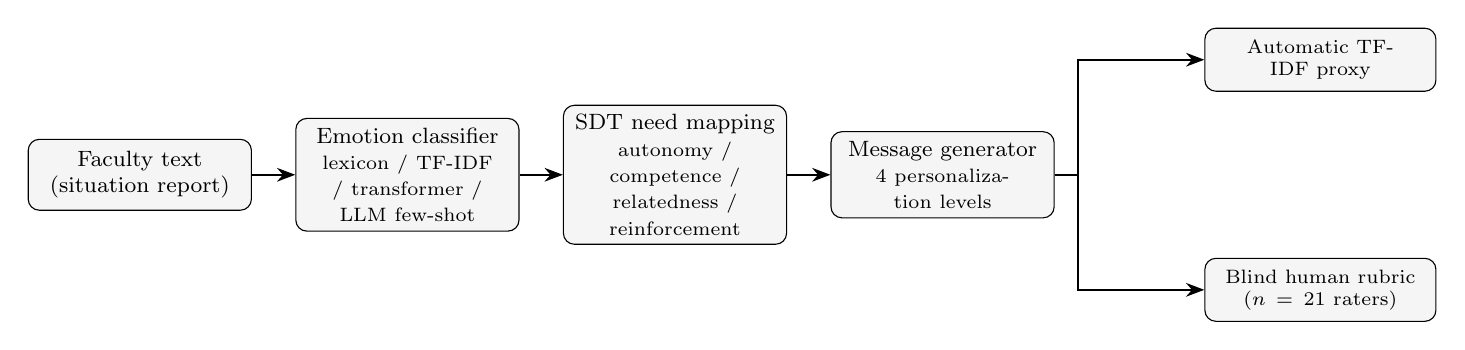
\begin{tikzpicture}[
  node distance=0.55cm,
  box/.style={rectangle, draw, rounded corners, align=center, minimum height=0.9cm, font=\footnotesize, fill=gray!8, text width=2.6cm},
  smallbox/.style={rectangle, draw, rounded corners, align=center, minimum height=0.8cm, font=\scriptsize, fill=gray!8, text width=2.7cm},
  arr/.style={-{Stealth}, thick}
]
\node[box] (text) {Faculty text\\ (situation report)};
\node[box, right=of text] (clf) {Emotion classifier\\ \scriptsize lexicon / TF-IDF / transformer / LLM few-shot};
\node[box, right=of clf] (need) {SDT need mapping\\ \scriptsize autonomy / competence / relatedness / reinforcement};
\node[box, right=of need] (gen) {Message generator\\ \scriptsize 4 personalization levels};
\node[smallbox, above right=0.5cm and 0.3cm of gen, xshift=1.6cm] (auto) {Automatic TF-IDF proxy};
\node[smallbox, below right=0.5cm and 0.3cm of gen, xshift=1.6cm] (human) {Blind human rubric\\ \scriptsize ($n=21$ raters)};
\draw[arr] (text) -- (clf);
\draw[arr] (clf) -- (need);
\draw[arr] (need) -- (gen);
\draw[arr] (gen.east) -- ++(0.3,0) |- (auto.west);
\draw[arr] (gen.east) -- ++(0.3,0) |- (human.west);
\end{tikzpicture}}
\caption{Pipeline used in all three experiments. Free text describing a work situation is classified for emotion by one of four classifier families (Section~\ref{sec:classifiers}); the predicted (or, in the oracle condition, gold) emotion is mapped to an SDT need (Section~\ref{sec:sdtmapping}); a message generator produces one of four personalization levels conditioned on that need and, at the most detailed level, on the original text; the resulting messages are scored by an automatic text-similarity proxy and by blind human raters (Sections~\ref{sec:automatic}--\ref{sec:human}).\label{fig:pipeline}}
%\end{adjustwidth}
\end{figure}

\subsection{Datasets}

Two public corpora supply the emotion-labeled text used to train and evaluate the classifiers in Experiment~1. GoEmotions \cite{demszky2020} contributes 58{,}000 English Reddit comments, of which single-label rows are retained and regrouped from the original 27 fine-grained categories into the Ekman-6-plus-neutral taxonomy using the mapping released with the dataset. ISEAR \cite{scherer1994} contributes roughly 7{,}600 self-reported emotional situations in seven categories; ISEAR is restricted here to the five categories it shares with the Ekman taxonomy (anger, disgust, fear, joy, sadness), dropping shame and guilt, which have no Ekman equivalent. No public, labeled corpus of higher-education faculty emotion exists at the time of writing -- a search for one was conducted before designing Experiment~2 and none was found -- which is why Experiment~2 (Section~\ref{sec:vignettes}) relies on a researcher-authored scenario set rather than a faculty-specific corpus, and why that set is described throughout this paper as a stress test, not a dataset of real faculty emotion.

\subsection{Emotion Classifiers}
\label{sec:classifiers}

Four classifier families of increasing semantic sophistication are evaluated on both corpora:
\begin{enumerate}
\item \textit{nrc\_lexicon} -- word counting against the NRC Emotion Lexicon \cite{mohammad2013}, the same class of method used in the closest prior teacher-emotion work \cite{chen2020}. The predicted label is the emotion with the most lexicon hits in a text; ties default to the majority class.
\item \textit{tfidf\_logreg} -- a TF-IDF vectorizer (unigrams and bigrams, 20{,}000 features, sublinear term-frequency scaling) feeding a logistic regression classifier with class-balanced weighting, trained on all seven GoEmotions categories.
\item \textit{transformer} -- \texttt{distilbert-base-uncased}, fine-tuned for three epochs (batch size 16, learning rate $2\times10^{-5}$) on all seven GoEmotions categories.
\item \textit{llm\_fewshot} -- an API call to an LLM (\texttt{claude-sonnet-4-6}) with five labeled in-context examples per class and no fine-tuning, used purely as a classifier (not as a generator) in this experiment.
\end{enumerate}

Because \textit{tfidf\_logreg} and \textit{transformer} are trained on all seven GoEmotions categories, they can predict \textit{neutral} or \textit{surprise} on the five-category ISEAR and vignette evaluations, where both labels are guaranteed wrong and structurally invisible in a same-label confusion matrix -- the corresponding rows simply undercount. We report this explicitly as an \emph{out-of-label-space rate} (the fraction of predictions falling outside the evaluation label set) and additionally fit \textit{tfidf\_logreg\_5class} and \textit{transformer\_5class}, the same algorithms restricted to the five shared categories at training time, as the fair, label-space-matched comparison against \textit{nrc\_lexicon} and \textit{llm\_fewshot}, both of which are already restricted to the evaluation label space by construction. Both versions are reported throughout: the seven-category variants as a realistic ``what happens if a model trained for a broader context is deployed into a narrower one'' baseline, and the five-category variants as the methodologically fair comparison point.

\subsection{Faculty Scenario Set}
\label{sec:vignettes}

Experiment~2 applies the same six classifier variants to 75 short, first-person vignettes written to operationalize eight stressor categories drawn from the qualitative literature on academic-staff burnout \cite{watts2011} and the task structure of the WTMST \cite{fernet2008}: workload overload, loss of autonomy, administrative pressure, lack of recognition, isolation, student disengagement, research--teaching conflict, and positive engagement (the last included as a non-distress control). Vignettes were written in sets of 15 per target emotion (anger, disgust, fear, sadness, joy -- the five categories shared with ISEAR), each tagged with the emotion it was written to express, a corresponding SDT need, and a stressor category. Table~\ref{tab:stressor-dist} and Figure~\ref{fig:stressor-dist} show how the 75 items distribute across the eight stressor categories; the distribution is intentionally balanced by target emotion (15 per emotion, Section~\ref{sec:vignettes}) rather than by stressor category, so administrative-pressure scenarios -- the largest single category -- appear across several emotions (e.g., anger at an imposed platform, fear of an unannounced audit), while narrower categories such as student disengagement are represented by a single illustrative item. Table~\ref{tab:example-messages} (Section~\ref{sec:sdtmapping}) shows two representative items. This set is a researcher-authored stress test, not a sample of real faculty communication; no faculty members were surveyed, observed, or recorded to produce it, and it is not presented as such anywhere in this paper. An optional expert face-validity check on the vignettes themselves (a separate instrument asking whether the described situation and assigned emotion are plausible) was prepared but had not been completed by independent raters at the time of writing; this is reported candidly as an open task rather than presenting unverified scenario validity as established.

\begin{table}[H]
\caption{Stressor-category distribution of the 75 vignettes.\label{tab:stressor-dist}}
\begin{tabularx}{\textwidth}{Xc}
\toprule
\textbf{Stressor Category} & \textbf{n (of 75)} \\
\midrule
Administrative pressure & 31 \\
Positive engagement (non-distress control) & 15 \\
Isolation & 9 \\
Lack of recognition & 6 \\
Loss of autonomy & 6 \\
Workload overload & 4 \\
Research--teaching conflict & 3 \\
Student disengagement & 1 \\
\bottomrule
\end{tabularx}
\end{table}

\begin{figure}[H]
\centering

\includegraphics[width=0.78\textwidth]{figures/vignette_stressor_distribution.png}
\caption{Stressor-category distribution of the 75 researcher-authored vignettes underlying Experiments~2--3 (Table~\ref{tab:stressor-dist}).\label{fig:stressor-dist}}
\end{figure}

\subsection{SDT Need Mapping and Intervention Generation}
\label{sec:sdtmapping}

Each emotion used in Experiments~1--2 is mapped to one of four categories used by the message generator: autonomy (anger, disgust -- both commonly follow a perceived unfair constraint or loss of control), competence (fear, surprise -- commonly follow a perceived threat to one's adequacy or a need for clarity), relatedness (sadness -- commonly follows social disconnection or a lack of recognition), and reinforcement (joy -- a need-satisfied state in which the appropriate response is to reinforce rather than to address a deficit). Table~\ref{tab:sdt-mapping} lists the full mapping with its rationale; neutral input maps to no specific need. This mapping is a literature-informed design choice, not an empirically validated instrument, and is flagged as such in Section~\ref{sec:limitations}.

\begin{table}[H]
\caption{Emotion-to-need mapping used by the message generator.\label{tab:sdt-mapping}}
\begin{tabularx}{\textwidth}{llX}
\toprule
\textbf{Emotion} & \textbf{SDT Need} & \textbf{Rationale} \\
\midrule
Anger & Autonomy & Commonly follows a perceived unfair constraint or loss of control over one's work. \\
Disgust & Autonomy & Often reflects a values-versus-autonomy conflict with imposed policies or practices. \\
Fear & Competence & Commonly reflects a perceived threat to one's adequacy (e.g., evaluation, failure, being replaced). \\
Surprise & Competence & Often follows unexpected feedback, related to a need for clarity. \\
Sadness & Relatedness & Commonly linked to social disconnection or lack of recognition. \\
Joy & Reinforcement & Needs already appear met; the appropriate response is to reinforce, not to address a deficit. \\
Neutral & None & No clear emotional signal detected. \\
\bottomrule
\end{tabularx}
\end{table}

Four message-personalization levels are generated for every vignette, forming the ablation at the center of Experiment~3:
\begin{enumerate}
\item \textit{generic} -- an identical message regardless of anything detected, used as the floor condition.
\item \textit{emotion\_only} -- acknowledges the raw detected emotion in one sentence, with no theoretical framing and no reference to the situation.
\item \textit{need\_only} -- routes through the mapped SDT need using a small set of hand-written templates phrased in the vocabulary of that need, without referencing the specific situation.
\item \textit{full\_context} -- generated by an LLM call given the SDT need and the full vignette text, instructed to reference a concrete detail of the situation; there is no template version of this level, since the entire point is content that a small fixed template set cannot express.
\end{enumerate}

Table~\ref{tab:example-messages} shows the four levels for two vignettes spanning different emotions and needs, drawn unedited from the experimental output. All four levels were generated in two conditions: \textit{oracle}, using the gold (researcher-assigned) emotion label, and \textit{end\_to\_end}, using the label predicted by \textit{llm\_fewshot} -- the best-performing classifier from Experiment~1 -- together with a \textit{need\_match\_rate} diagnostic recording how often a misclassified emotion nonetheless maps to the correct SDT need (anger and disgust, for example, both map to autonomy, so not every classification error degrades the downstream message).

\begin{table}[H]
\caption{Example generated messages by personalization level, for two representative vignettes (drawn unedited from experimental output).\label{tab:example-messages}}
\begin{tabularx}{\textwidth}{lX}
\toprule
\multicolumn{2}{l}{\textbf{Vignette V1} (anger $\rightarrow$ autonomy; stressor: workload overload)} \\
\multicolumn{2}{p{\dimexpr\textwidth-2\tabcolsep\relax}}{\footnotesize ``I was assigned three additional committees without being consulted, on top of an already full teaching load.''} \\
\midrule
\textit{generic} & Thank you for sharing how things are going. Keep up the great work, you are doing fine! \\
\textit{emotion\_only} & It's understandable to feel angry about this. \\
\textit{need\_only} & It sounds like a decision was made without your input. What is one part of this you could still shape on your own terms? \\
\textit{full\_context} & Having three committees added to an already full teaching load -- without even being asked -- is genuinely a lot to carry. Your time and voice matter here. It's okay to advocate for boundaries; doing so isn't selfish, it's sustainable. \\
\midrule
\multicolumn{2}{l}{\textbf{Vignette V2} (sadness $\rightarrow$ relatedness; stressor: isolation)} \\
\multicolumn{2}{p{\dimexpr\textwidth-2\tabcolsep\relax}}{\footnotesize ``Nobody on the faculty has asked how I am doing since I came back from sick leave.''} \\
\midrule
\textit{generic} & Thank you for sharing how things are going. Keep up the great work, you are doing fine! \\
\textit{emotion\_only} & It sounds like that's been a difficult, disheartening experience. \\
\textit{need\_only} & Your work seems to be going unnoticed right now, and that is worth naming. Who would you want to know about it? \\
\textit{full\_context} & Returning from sick leave and feeling invisible to colleagues is genuinely hard -- you deserved a warm welcome back. Your presence on that faculty matters, and I hope someone reaches out soon. You shouldn't have to navigate this return alone. \\
\bottomrule
\end{tabularx}
\end{table}

\subsection{Automatic Evaluation}
\label{sec:automatic}

As a cheap, reproducible sanity check, each generated message is scored by cosine similarity, in a shared TF-IDF space fit jointly over all messages and need descriptions, to the textual description of its target SDT need. This metric is reported throughout as a secondary proxy, not the primary outcome, for a reason demonstrated directly in Section~\ref{sec:divergence}: it is structurally biased toward messages that share abstract need-vocabulary with the need description and against messages that achieve the same intent through concrete, situation-specific language -- exactly the trade made by the \textit{full\_context} level.

\subsection{Human Evaluation Protocol}
\label{sec:human}

The primary outcome of Experiment~3 is a blind expert rating exercise. Twenty-one higher-education faculty and researchers (Table~\ref{tab:raters}) each rated a stratified subsample of 25 vignettes (5 per emotion category), with up to four anonymized message slots per vignette -- one per personalization level, randomly ordered and labeled A--D so that raters could not infer which level produced which message -- on four dimensions: \textit{relevance} (does the message respond to what was described), \textit{specificity} (does it engage with concrete detail rather than generic language), \textit{SDT alignment} (does it support the need the message was theoretically designed to support, described to raters in plain language rather than as SDT terminology), and \textit{motivational usefulness} (would the rater expect this message to be motivating if they received it). Each dimension was rated on a 1--5 scale. Ratings were collected via a Google Forms instrument; the raw, de-identified export (no name, email, or other identifying field) and one CSV per rater accompany this paper (see Data Availability Statement). This was an expert content-rating exercise on synthetic, machine-generated text, not a study of any individual's own emotional state, consistent with the determination reported in the Institutional Review Board Statement below.

\begin{table}[H]
\caption{Human-rater composition ($n=21$).\label{tab:raters}}
\begin{tabularx}{\textwidth}{XCC}
\toprule
\textbf{Role} & \textbf{n} & \textbf{Years of Experience} \\
\midrule
Professor & 6 & $>$20 \\
Associate Professor & 10 & 10--20 \\
Assistant Professor & 3 & 5--10 \\
Researcher & 2 & 5--10 \\
\midrule
Total & 21 & -- \\
\bottomrule
\end{tabularx}
\end{table}

\subsection{Statistical Analysis}
\label{sec:statanalysis}

The automatic ablation metric (Section~\ref{sec:automatic}) is item-level by construction (one TF-IDF similarity score per vignette per condition), so its staircase comparisons between adjacent personalization levels (\textit{generic} vs.\ \textit{emotion\_only}, \textit{emotion\_only} vs.\ \textit{need\_only}, \textit{need\_only} vs.\ \textit{full\_context}) are tested directly with paired $t$-tests across the 75 vignettes, supported by the Wilcoxon signed-rank test as a non-parametric check, and summarized with Cohen's $d$.

The human rubric (Section~\ref{sec:human}) requires more care, because the 525 ratings nominally available per personalization level per dimension ($21$ raters $\times$ $25$ vignettes) are not 525 independent observations: ratings produced by the same rater are correlated with one another in ways a naive item-level test does not model, and treating them as independent risks an anti-conservative (too easily significant) result. Three statistics are therefore reported for every staircase comparison, in increasing order of how much non-independence they account for: (i) a naive item-level paired $t$-test across all 525 rater-by-vignette observations, reported only as a descriptive baseline; (ii) a rater-level aggregated paired $t$-test and Wilcoxon signed-rank test, in which each of the $n=21$ raters' 25 item-level ratings are first averaged within level and dimension, so the test is conducted on 21, not 525, paired observations, with Cohen's $d$ computed on these by-rater differences; and (iii) a crossed mixed-effects linear model (score regressed on personalization level as a fixed effect, with crossed random intercepts for rater and for vignette, fit by restricted maximum likelihood, REML), refit three times with the reference level releveled so that all three adjacent-step contrasts are estimated directly with their own standard errors. Statistic (ii) is treated as the primary confirmatory result throughout Section~\ref{sec:human-results}, since it makes the fewest distributional assumptions about the rater/vignette structure; statistic (iii) is reported as a model-based robustness check. Inter-rater agreement on raw item-level scores is additionally summarized with pairwise Pearson correlation; Section~\ref{sec:limitations} notes that the intraclass correlation coefficient (ICC) would be a preferable statistic for a confirmatory follow-up. Classifier accuracy is reported against a majority-class baseline throughout, so that absolute accuracy figures are interpretable relative to a trivial reference point rather than in isolation.

\subsection{Use of Generative AI}

Two parts of this study's experimental material were generated by a large language model rather than written by hand, and both are disclosed here rather than only in passing. First, the \textit{llm\_fewshot} classifier (Section~\ref{sec:classifiers}) and the \textit{full\_context} personalization level (Section~\ref{sec:sdtmapping}) both call an LLM (\texttt{claude-sonnet-4-6}, Anthropic) as part of the experimental pipeline itself -- this is a methods choice under test, not writing assistance, and its outputs are the object of evaluation in Sections~\ref{sec:domainshift}--\ref{sec:divergence}, not incidental text. Second, the author used a large language model (Claude, Anthropic) as a drafting and editing aid in preparing this manuscript from the underlying code, data, and results; all reported numbers were generated by the analysis code in the accompanying repository, and the author reviewed the manuscript text and takes full responsibility for its content and for the accuracy of all reported figures. No experimental data -- classifier predictions, human ratings, or generated messages -- were altered, paraphrased, or summarized by the language model in a way that bypasses the underlying logged outputs; all reported statistics were recomputed directly from those logs.

\section{Results}

\subsection{Domain-Shift Ladder}
\label{sec:domainshift}

Table~\ref{tab:domain-shift} and Figure~\ref{fig:domain-shift} report accuracy for all six classifier variants on three test conditions of increasing distance from the GoEmotions training distribution: in-domain (GoEmotions test split, seven categories), cross-dataset (ISEAR, five shared categories), and near-domain (the 75 faculty vignettes, five shared categories).

\begin{table}[H]
\caption{Classifier accuracy across domain shift. ``5class'' variants are trained only on the five categories shared with ISEAR and the vignette set.\label{tab:domain-shift}}
\begin{tabularx}{\textwidth}{lCCC}
\toprule
\textbf{Model} & \textbf{GoEmotions (In-Domain)} & \textbf{ISEAR (Cross-Dataset)} & \textbf{Vignettes (Near-Domain)} \\
\midrule
Majority-class baseline & 0.350 & 0.200 & 0.200 \\
nrc\_lexicon & 0.384 & 0.326 & 0.360 \\
tfidf\_logreg (7-class) & 0.599 & 0.259 \textsuperscript{a} & 0.227 \textsuperscript{b} \\
tfidf\_logreg\_5class (fair) & n/a & 0.381 & 0.387 \\
transformer (7-class) & \textbf{0.693} & 0.338 \textsuperscript{c} & 0.347 \textsuperscript{d} \\
transformer\_5class (fair) & n/a & 0.545 & 0.520 \\
llm\_fewshot & 0.467 & \textbf{0.785} & \textbf{0.893} \\
\bottomrule
\end{tabularx}
\noindent{\footnotesize{\textsuperscript{a} 46.5\% of predictions fell outside the 5-label evaluation space. \textsuperscript{b} 49.3\% out-of-label-space. \textsuperscript{c} 54.4\% out-of-label-space. \textsuperscript{d} 52.0\% out-of-label-space. All out-of-label-space predictions are guaranteed incorrect and are not visible in a same-label confusion matrix.}}
\end{table}

\begin{figure}[H]
\centering

\includegraphics[width=0.85\textwidth]{figures/domain_shift_ladder.png}
\caption{Classifier accuracy across three test conditions of increasing distance from the GoEmotions training distribution. ``5class'' variants are restricted to the five emotion categories shared with ISEAR and the vignette set; the non-suffixed \textit{tfidf\_logreg} and \textit{transformer} bars are trained on all seven GoEmotions categories and are not label-space-matched to the cross-dataset and near-domain evaluations (Section~\ref{sec:domainshift}).\label{fig:domain-shift}}
\end{figure}

Three patterns are visible. First, on the label-space-fair comparisons (\textit{nrc\_lexicon}, the two \textit{\_5class} variants, and \textit{llm\_fewshot}), accuracy degrades from lexicon counting through TF-IDF to a fine-tuned transformer to LLM few-shot exactly as current NLP practice would predict, with no surprises -- itself a useful check that the fairness correction did not introduce a new artifact. Second, in-domain performance is not a safe proxy for out-of-domain performance, and the relationship can invert: the seven-category transformer achieves the best in-domain accuracy of any non-LLM method (0.693) but also the highest out-of-label-space rate on the cross-dataset evaluation (54.4\%, exceeding even the seven-category TF-IDF model's 46.5\%) -- a better fit to the training distribution made the model more, not less, confident in wrong, in-domain-typical predictions once the distribution shifted. Third, \textit{llm\_fewshot} is the only method in this comparison that is robust to domain shift without any fine-tuning step, and it is also the worst-performing method in-domain (0.467, against 0.599 and 0.693 for the supervised classical and transformer models) -- it has nothing to overfit to GoEmotions' noisy, short, sarcasm-prone Reddit register, which is a real cost in-domain and an advantage once the register changes.

The label-space correction matters substantively, not just as a footnote. Before restricting \textit{tfidf\_logreg} and \textit{transformer} to the five shared categories, the original (seven-category) comparison suggested that simple lexicon counting generalized better cross-domain than supervised TF-IDF (0.326 vs.\ 0.259 on ISEAR). Once both methods are evaluated on a matched label space, the conclusion reverses: \textit{tfidf\_logreg\_5class} outperforms \textit{nrc\_lexicon} on both out-of-domain tests (0.381 vs.\ 0.326 on ISEAR; 0.387 vs.\ 0.360 on the vignettes). Close to half of the original \textit{tfidf\_logreg} model's cross-domain predictions (46.5\% on ISEAR, 49.3\% on the vignettes) fell into label categories -- \textit{neutral}, \textit{surprise} -- that do not exist in either evaluation set and were therefore guaranteed wrong; the earlier, unfair comparison was measuring this artifact at least as much as it was measuring genuine semantic generalization.

\subsection{Per-Emotion Error Analysis}

Table~\ref{tab:per-emotion} breaks down vignette accuracy by emotion for the four label-space-fair classifiers. Disgust is the most consistently difficult category for every non-LLM method: \textit{nrc\_lexicon} and \textit{tfidf\_logreg\_5class} confuse it most often with anger (8/15 and 5/15 vignettes, respectively), and \textit{tfidf\_logreg\_5class} and \textit{transformer\_5class} fail to recognize it at all (0\% accuracy), more often mistaking it for sadness or anger than for any other class. Sadness is the second-most difficult category for the classical methods (13.3\% for \textit{nrc\_lexicon}) before improving substantially for the transformer (60\%). \textit{llm\_fewshot} is the only method that resolves both categories well (60\% on disgust, its single weakest class; 100\% on sadness, tied for its best), and its few errors on disgust are concentrated in the same disgust-to-anger confusion seen in the weaker methods (6 of 15 disgust vignettes), suggesting this confusion reflects a genuinely difficult linguistic distinction in this register -- both emotions are frequently expressed through similar complaint-like language about being treated unfairly -- rather than a weakness specific to one method. Figure~\ref{fig:confusion-panel} contrasts the confusion matrix of the weakest method (\textit{nrc\_lexicon}) against the strongest (\textit{llm\_fewshot}) on the vignette set.

\begin{table}[H]
\caption{Per-emotion accuracy on the 75-item vignette set, label-space-fair classifiers only.\label{tab:per-emotion}}
\small
\begin{tabularx}{\textwidth}{lCCCC}
\toprule
\textbf{Emotion} & \textbf{nrc\_lexicon} & \textbf{tfidf\_logreg\_5class} & \textbf{transformer\_5class} & \textbf{llm\_fewshot} \\
\midrule
Anger & 0.600 & 0.467 & 0.333 & 0.867 \\
Disgust & 0.133 & 0.000 & 0.000 & 0.600 \\
Fear & 0.467 & 0.467 & 0.733 & 1.000 \\
Joy & 0.467 & 0.533 & 0.933 & 1.000 \\
Sadness & 0.133 & 0.467 & 0.600 & 1.000 \\
\midrule
Overall & 0.360 & 0.387 & 0.520 & 0.893 \\
\bottomrule
\end{tabularx}
\end{table}

\begin{figure}[H]
\begin{adjustwidth}{-\extralength}{0cm}
\centering
\subfloat[\centering nrc\_lexicon]{
\includegraphics[width=7.5cm]{figures/nrc_lexicon_vignettes_cm.png}}
\subfloat[\centering llm\_fewshot]{
\includegraphics[width=7.5cm]{figures/llm_fewshot_vignettes_cm.png}}
\end{adjustwidth}
\caption{Confusion matrices on the 75-item vignette set for the weakest (\textbf{a}) and strongest (\textbf{b}) classifier in the label-space-fair comparison. Both share a tendency to misclassify disgust as anger; \textit{llm\_fewshot} resolves every other category at or near ceiling.\label{fig:confusion-panel}}
\end{figure}

\subsection{Automatic Ablation Results}
\label{sec:autoablation}

Table~\ref{tab:auto-ablation} and Figure~\ref{fig:ablation} report the TF-IDF similarity-to-need-description proxy across the four personalization levels, in both the oracle and end-to-end conditions. In both conditions, the jump from \textit{generic} to \textit{emotion\_only} is small and, in the oracle condition, not statistically significant (mean difference 0.0039, $p=0.269$); the jump from \textit{emotion\_only} to \textit{need\_only} is the largest step in the oracle condition (mean difference 0.027, $p<0.0001$, Cohen's $d=0.55$) and a significant but smaller step end-to-end (mean difference 0.018, $p=0.005$); and the jump from \textit{need\_only} to \textit{full\_context} is not significant in either condition (oracle: $p=0.083$; end-to-end: $p=0.518$), with \textit{full\_context} scoring numerically below \textit{need\_only} in both. Read in isolation, this metric would support the conclusion that SDT-need-routing is valuable but that adding full situational context adds nothing further, or even costs a small amount of automatic-metric-measured relevance. Section~\ref{sec:divergence} shows why that reading does not survive contact with human judgment.

\begin{table}[H]
\caption{Automatic TF-IDF similarity-to-need-description proxy by personalization level.\label{tab:auto-ablation}}
\begin{tabularx}{\textwidth}{lCC}
\toprule
\textbf{Level} & \textbf{Oracle (Mean Sim.)} & \textbf{End-to-End (Mean Sim.)} \\
\midrule
generic & 0.0229 & 0.0229 \\
emotion\_only & 0.0267 (n.s.) & 0.0313 (*) \\
need\_only & 0.0541 (***) & 0.0491 (**) \\
full\_context & 0.0455 (n.s.) & 0.0461 (n.s.) \\
\bottomrule
\end{tabularx}
\noindent{\footnotesize{Significance markers compare each level to the row immediately above (paired $t$-test): n.s.\ $p\geq0.05$; * $p<0.05$; ** $p<0.01$; *** $p<0.0001$. Exact $p$-values: generic$\rightarrow$emotion\_only oracle $p=0.269$, end-to-end $p=0.013$; emotion\_only$\rightarrow$need\_only oracle $p<0.0001$, end-to-end $p=0.005$; need\_only$\rightarrow$full\_context oracle $p=0.083$, end-to-end $p=0.518$.}}
\end{table}

\begin{figure}[H]
\begin{adjustwidth}{-\extralength}{0cm}
\centering
\subfloat[\centering Oracle condition]{
\includegraphics[width=7.5cm]{figures/exp3_ablation_oracle.png}}
\subfloat[\centering End-to-end condition]{
\includegraphics[width=7.5cm]{figures/exp3_ablation_end_to_end.png}}
\end{adjustwidth}
\caption{Automatic TF-IDF-similarity-to-need-description proxy across the four personalization levels, using the gold emotion label (\textbf{a}, oracle) or the label predicted by \textit{llm\_fewshot} (\textbf{b}, end-to-end). Error bars show bootstrap confidence intervals. Section~\ref{sec:divergence} shows that this metric disagrees with human judgment about the value of the \textit{full\_context} level.\label{fig:ablation}}
\end{figure}

\subsection{Human Evaluation Results}

Twenty-one raters (Table~\ref{tab:raters}) each rated up to four message slots across 25 stratified vignettes on four dimensions, yielding 525 item-level ratings per personalization level per dimension, which collapse to 21 by-rater means per level per dimension once aggregated as described in Section~\ref{sec:statanalysis}. Figure~\ref{fig:human-staircase} and Table~\ref{tab:human-staircase} show a clean, monotonic staircase on the raw means: every personalization level outperforms the one before it, on every one of the four dimensions, with no exceptions across all 21 raters and 25 items. Whether each of those three steps is \emph{statistically} robust, however, depends on which of the three statistics from Section~\ref{sec:statanalysis} is used, which is the focus of the rest of this subsection.

\begin{figure}[H]
\centering

\includegraphics[width=0.85\textwidth]{figures/human_rubric_staircase.png}
\caption{Mean human expert rating (1--5 scale; $n=21$ raters $\times$ 25 stratified vignettes = 525 ratings per bar) by personalization level and rating dimension. Every level outperforms the one before it on every dimension, with no exceptions; the largest single step is \textit{need\_only} to \textit{full\_context} (Section~\ref{sec:human-results}), the opposite of what the automatic metric in Figure~\ref{fig:ablation} suggests.\label{fig:human-staircase}}
\end{figure}

\begin{table}[H]
\caption{Human expert rating means by personalization level and dimension ($n=525$ item-level ratings per cell; equivalently, the mean of 21 by-rater means).\label{tab:human-staircase}}
\begin{tabularx}{\textwidth}{lCCCC}
\toprule
\textbf{Level} & \textbf{Relevance} & \textbf{Specificity} & \textbf{SDT Alignment} & \textbf{Motivational Usefulness} \\
\midrule
generic & 2.47 & 2.45 & 2.44 & 2.47 \\
emotion\_only & 2.83 & 2.71 & 2.77 & 2.86 \\
need\_only & 2.89 & 2.91 & 2.90 & 2.99 \\
full\_context & \textbf{3.52} & \textbf{3.49} & \textbf{3.43} & \textbf{3.44} \\
\bottomrule
\end{tabularx}
\noindent{\footnotesize{Significance of each step is assessed three ways in the text (Section~\ref{sec:human-results}): a naive item-level test ($n=525$), a rater-level aggregated test ($n=21$, primary), and a crossed mixed-effects model. The three do not always agree; see Figure~\ref{fig:effect-size} and the discussion below.}}
\end{table}
\label{sec:human-results}

Two comparisons matter most, and the two differ sharply in how robust they are once rater-level non-independence is taken into account.

The \textit{emotion\_only}-to-\textit{need\_only} step -- the SDT-routing step -- is the more fragile of the two. In the naive item-level analysis it reaches significance on three of four dimensions (specificity, SDT alignment, motivational usefulness); in the rater-level aggregated analysis ($n=21$, the primary statistic), only the specificity gain clearly survives (mean difference 0.196, $t(20)=3.15$, $p=0.005$, $d=0.69$), while SDT alignment ($p=0.060$) and motivational usefulness ($p=0.090$) drop to borderline/non-significant, and relevance remains non-significant under both treatments (item-level $p=0.298$; rater-level $p=0.367$). The crossed mixed-effects model tells essentially the same story: significant for specificity ($p=0.0046$), borderline for SDT alignment and motivational usefulness ($p\approx0.048$ for both), and not significant for relevance ($p=0.372$). Two independent, more conservative statistical treatments therefore agree that naming the underlying SDT need reliably helps raters perceive a message as more specific, but its effect on perceived theoretical alignment, motivational usefulness, and overall relevance is, at best, modest and is not robustly demonstrated by this sample once pseudo-replication is corrected for.

The \textit{need\_only}-to-\textit{full\_context} step is, by contrast, the most robust finding in the whole staircase. It is the largest jump on every dimension in the naive item-level analysis (relevance: mean difference 0.634, $d=0.40$; specificity: 0.581, $d=0.34$; SDT alignment: 0.535, $d=0.35$; motivational usefulness: 0.450, $d=0.32$; all $p<0.0001$); it remains significant on every dimension in the rater-level analysis (relevance: $d=0.71$, $p=0.004$; specificity: $d=0.48$, $p=0.041$; SDT alignment: $d=0.70$, $p=0.004$; motivational usefulness: $d=0.72$, $p=0.004$); and the crossed mixed-effects model agrees, with every coefficient significant beyond $p<10^{-10}$. This is the central, best-supported empirical answer to the question posed in Section~1: grounding a generated message in the faculty member's specific reported situation, on top of SDT-need-routing, improves perceived message quality more reliably than SDT-routing does on its own -- a more carefully qualified claim than asserting that emotion recognition is simply ``outperformed,'' and one that survives the more conservative of two independent statistical treatments rather than resting on the naive analysis alone.

\begin{figure}[H]
\centering

\includegraphics[width=0.78\textwidth]{figures/human_rubric_effect_size_staircase.png}
\caption{Effect size (Cohen's $d$, rater-level paired differences, $n=21$) of each of the three staircase steps, by rating dimension. Significance markers (paired $t$-test on by-rater means): n.s.\ $p\geq0.05$; * $p<0.05$; ** $p<0.01$. The \textit{need\_only}$\to$\textit{full\_context} step (right) is large and significant on every dimension; the \textit{emotion\_only}$\to$\textit{need\_only} step (center) is significant only for specificity.\label{fig:effect-size}}
\end{figure}

Pairwise inter-rater correlation on raw item-level scores is low throughout (0.05--0.12 across levels and dimensions), indicating that individual raters do not strongly agree on the absolute 1--5 score assigned to a given message -- plausibly a matter of differing personal calibration of the scale rather than disagreement about relative ordering. This low agreement is precisely why the rater-level and mixed-effects analyses above, rather than the naive item-level analysis, are treated as the load-bearing statistics in this paper: low inter-rater agreement is a direct symptom of the non-independence those two methods correct for. Section~\ref{sec:limitations} reports the remaining caveats honestly rather than omitting them.

\subsection{Automatic-vs-Human Divergence}
\label{sec:divergence}

The automatic metric (Section~\ref{sec:domainshift}) and the human ratings (Section~\ref{sec:human-results}) tell different, even contradictory, stories about the value of the \textit{full\_context} level: the automatic metric finds no significant gain over \textit{need\_only} and a numerically lower score in both conditions; the human raters find the largest, most robust gain in the entire staircase, on every dimension, under every statistical treatment used. The discrepancy has an identifiable mechanical cause. The \textit{need\_only} messages are a small set of hand-written templates deliberately phrased close to the SDT need-description vocabulary (Table~\ref{tab:sdt-mapping}), because the need descriptions used to compute the automatic score were themselves written in similar abstract language. The \textit{full\_context} messages are LLM-generated, unique per vignette, and reference a concrete detail of the specific situation -- for example, naming the precise number of committees added to a workload, rather than referring generically to a loss of autonomy. The automatic metric rewards lexical overlap with an abstract need description; concrete specificity is precisely the property that \textit{full\_context} trades that lexical overlap away for. This is not a contradiction to be explained away -- it is direct, internally consistent evidence that a text-similarity proxy is not a safe substitute for human judgment when evaluating which of two generated messages is actually better, and it is the reason this study leads with the human rubric, not the automatic score, as its primary result.

\subsection{Summary of Evidence}

Table~\ref{tab:rq-summary} maps each research question raised in Sections~1--2 onto the experiment that addresses it, the evidence obtained, and the resulting conclusion, stated at the level of confidence the evidence actually supports.

\begin{table}[H]
\begin{adjustwidth}{-\extralength}{0cm}
\caption{Research questions, the experiment addressing each, the evidence obtained, and the resulting conclusion.\label{tab:rq-summary}}
\begin{tabularx}{\fulllength}{XXXX}
\toprule
\textbf{Research Question} & \textbf{Experiment} & \textbf{Evidence} & \textbf{Conclusion} \\
\midrule
How does classifier choice affect robustness to domain shift, and is a simple lexicon method really more robust than supervised TF-IDF, as an unfair comparison suggests? & Exp.\ 1 (Section~\ref{sec:domainshift}) & Label-space-fair accuracy on GoEmotions/ISEAR/vignettes (Table~\ref{tab:domain-shift}); 46.5--54.4\% out-of-label-space rate for unfair 7-class models & The sophistication ladder (lexicon $<$ TF-IDF $<$ transformer $<$ LLM few-shot) holds once compared fairly; the original ``lexicon generalizes better'' finding was largely a label-space artifact. \\
\midrule
Which emotions remain hard to classify in faculty-like text, and for which methods? & Exp.\ 2 (Section~4.2) & Per-emotion accuracy, four fair classifiers (Table~\ref{tab:per-emotion}) & Disgust is the most consistently difficult category for every non-LLM method; \textit{llm\_fewshot} resolves it best but not perfectly. \\
\midrule
Does routing a detected emotion through an SDT need improve message quality more than detecting the emotion alone, on a cheap automatic proxy? & Exp.\ 3, automatic (Section~4.3) & TF-IDF similarity-to-need-description, oracle \& end-to-end (Table~\ref{tab:auto-ablation}) & SDT-routing helps on this proxy; adding situational grounding does not -- a conclusion later shown to be a metric artifact (Section~\ref{sec:divergence}). \\
\midrule
Does the same routing step improve message quality in blind expert judgment, and does that hold once rater-level non-independence is corrected for? & Exp.\ 3, human (Section~\ref{sec:human-results}) & 21-rater blind rubric; naive item-level, rater-level aggregated, and crossed mixed-effects analyses (Figure~\ref{fig:effect-size}) & SDT-routing alone is real but fragile (robust only for specificity); grounding the message in the specific situation, on top of SDT-routing, is the largest and most robust gain in the entire staircase under every statistical treatment used. \\
\midrule
Do automatic and human evaluation agree about which generated message is better? & Exp.\ 3, both (Section~\ref{sec:divergence}) & Direct comparison of Tables~\ref{tab:auto-ablation} and~\ref{tab:human-staircase} & No: the automatic metric and blind human judgment disagree specifically about the value of situational grounding, for an identifiable, mechanistic reason. \\
\bottomrule
\end{tabularx}
\end{adjustwidth}
\end{table}

\section{Discussion}

The central finding of this study is best stated narrowly: across two independent, more conservative statistical treatments of the human ratings (Section~\ref{sec:human-results}), grounding a generated message in the faculty member's specific reported situation, on top of SDT-need-routing, is the step that most reliably improves perceived message quality. SDT-need-routing by itself is a real but smaller and more fragile effect, surviving the stricter rater-level and mixed-effects analyses consistently only for the specificity dimension. Both results are broadly consistent with Self-Determination Theory \cite{deciryan2000} read as a design principle: autonomy, competence, and relatedness are the theory's operative constructs, not raw affect, so a message that engages one of them by name should help at least somewhat, and a message that engages it concretely, in the person's own terms, should help more. The pattern observed here -- a modest, partly fragile gain from naming the need, and a larger, robust gain from grounding it in detail -- is itself informative about how to apply SDT to message design: the theory's vocabulary alone is a weaker design lever than the theory's vocabulary combined with situational specificity.

The larger, robust step sits squarely within a separate, well-established literature on supportive communication. A meta-analysis of 23 studies on verbal person-centeredness in human support messages found a consistent positive association between how concretely a message engages with a person's specific situation and both the actual and perceived effectiveness of that message \cite{highdillard2012}. More directly relevant, an experimental study using a fictional computer program (``ListenerBot'') to deliver support messages of varying person-centeredness found that participants receiving more person-centered, situationally specific computer-generated feedback reported a greater reduction in emotional distress than those receiving generic feedback \cite{rains2020}. The finding reported here is consistent with both literatures and extends them to a different population (university faculty) and a different generation mechanism (an LLM conditioned on free text, rather than a human-authored or template-selected message).

The mechanism generating that situational detail is itself part of a fast-moving line of NLP research on LLM-produced supportive text. Zheng et al.\ \cite{zheng2024} use an LLM to generate richer self-chat training data specifically to make a small, deployable emotional-support chatbot more responsive to situational nuance -- a different mechanism aimed at a property similar to the one isolated here. The present results add a controlled, ablation-based estimate of how much that property is actually worth in human judgment relative to theory-routing alone, a question generation-focused work in that literature does not typically ask.

Two methodological results matter beyond this specific pipeline. The first concerns benchmarking practice: the label-space-fairness correction in Experiment~1 reversed an apparent finding (Section~\ref{sec:domainshift}) that a simpler lexicon method generalized better cross-domain than supervised TF-IDF. That apparent finding was, on inspection, almost half artifact -- a large fraction of the unfair model's cross-domain predictions fell into label categories that could not exist in the evaluation set by construction. Anyone building a similar pipeline cheaply on public data, where the training label space and the deployment label space rarely match exactly, should expect this kind of artifact by default and report an out-of-label-space rate alongside accuracy, not after the fact.

The second concerns evaluation practice for generated text more broadly. The divergence documented in Section~\ref{sec:divergence} between a text-similarity proxy and blind human judgment is a specific instance of a more general, recognized problem: automatic NLG metrics built on lexical or surface overlap are known to correlate poorly with human judgment of quality on exactly the dimensions -- specificity, appropriateness to context -- that distinguish good generated text from merely fluent generated text \cite{sai2022}. This caution is not specific to lexical-overlap metrics: even an LLM-based evaluator explicitly designed for closer human alignment reaches a Spearman correlation of only about 0.51 with human judgment on a standard summarization benchmark \cite{liu2023geval}, well short of the agreement a deployment decision would ideally rest on. The lesson generalizes past the one metric used here: automatic proxies for generated-text quality, lexical or LLM-based, are a sanity check that a generation pipeline has not broken, not a substitute for the kind of blind rater study this paper treats as primary.

For institutional practice, this study speaks most directly to faculty development and human-resources functions, not to clinical or counseling services. A growing body of organizational research treats digital-environment design itself as an SDT-relevant intervention: a recent survey of 482 university faculty found that institutional digital transformation predicts faculty performance partly through its effect on faculty's sense of competence (digital self-efficacy) \cite{sunyoon2025} -- the same theoretical logic this study applies at the level of a single generated message rather than an institution-wide program. Read together, the two studies suggest a coherent design principle for faculty-support technology at any scale: interventions earn their effect by supplying a specific psychological need, not by being digital, personalized, or AI-powered in some generic sense. A faculty-development office considering a tool like the one prototyped here should treat it as one input among several -- alongside workload data, peer mentoring, and existing wellbeing programming \cite{watts2011} -- not as a replacement for any of them, and should evaluate it the way this study does, against blind expert or end-user judgment of message quality, not only against engagement metrics or cost.

A specific risk deserves explicit treatment, because it is the most likely way a tool like this would be misused: routing a detected emotion to an automatically generated supportive message is not, and should not be marketed or deployed as, automated psychological diagnosis or therapy. A recent evaluation of LLM-based systems explicitly positioned as therapists found that they can express stigma toward mental health conditions and respond inappropriately or unsafely in crisis scenarios, with no clear improvement from newer or larger models \cite{moore2025}. The pipeline in this study differs from that use case in scope -- it classifies a coarse emotion category and generates one short supportive message, not a sustained therapeutic interaction -- but the same caution applies in miniature. An institution adopting this kind of design pattern should keep the tool's stated function narrow (acknowledging a reported situation and pointing toward a specific, named need), should route any signal of acute distress or crisis language to a human contact -- a department chair, an employee-assistance program, a wellbeing office -- rather than to the automated message generator, should avoid presenting the tool's output as a clinical judgment about the user's mental state, and should not retain individual-level emotional profiles beyond what the faculty member has explicitly consented to. None of this is a property the present feasibility study can validate; it is a design constraint that the study's own scope (Section~\ref{sec:limitations}) makes necessary to state plainly rather than leave implicit.

That practical reading carries the same caveat already noted in the Results: classifier accuracy on the near-domain vignette set, while best for \textit{llm\_fewshot} (0.893), remains well short of what most institutions would consider acceptable for an unsupervised, deployed system making decisions about a real faculty member's emotional state, and the personalization pipeline itself has only been tested on synthetic scenarios rated by external experts, not on real faculty interacting with the tool. This study is evidence for a design choice within a future system -- and, per the paragraph above, for how that future system's scope should be bounded -- not evidence that the system is ready to deploy.

\section{Limitations and Future Work}
\label{sec:limitations}

Several limitations bound how far these results should be generalized.

No data from real faculty members were collected or used at any stage of Experiments~2--3; the 75-item scenario set is researcher-authored, and although an instrument for an independent expert face-validity check on the vignettes themselves was prepared (Section~\ref{sec:vignettes}), it had not been completed at the time of writing. Readers should treat Experiment~2 as evidence about classifier behavior on a researcher-constructed stress test resembling plausible faculty language, not as evidence about real faculty communication.

The emotion-to-SDT-need mapping (Table~\ref{tab:sdt-mapping}) is a literature-informed design proposal, not an instrument that has itself been validated against, for example, expert ratings or faculty self-report; a useful next step would be to have organizational psychologists or faculty-development specialists review and, if necessary, revise the mapping before it is used in any deployed system.

Inter-rater agreement on the human rubric (Section~\ref{sec:human-results}) was low at the item level (pairwise Pearson $r$ of 0.05--0.12), and the rater pool, while professionally appropriate (Table~\ref{tab:raters}), was a convenience sample recruited through the authors' professional network rather than a representative sample of higher-education faculty internationally. The rater-level aggregated analysis and crossed mixed-effects model (Section~\ref{sec:statanalysis}) partially address the resulting non-independence and already changed one substantive conclusion (the SDT-routing step's robustness, Section~\ref{sec:human-results}); they do not, however, substitute for a larger and more diverse rater pool, and the intraclass correlation coefficient, computed on such a pool, would still be a more informative agreement statistic than the pairwise correlation used here.

The divergence between automatic and human evaluation (Section~\ref{sec:divergence}) was diagnosed for one specific similarity-based metric computed against one specific kind of reference text (a short need description). The argument that automatic metrics are an unsafe substitute for human judgment in this domain almost certainly generalizes beyond this exact metric, but alternative automatic metrics (e.g., neural embedding similarity) that might partially close the gap were not tested, and this metric is not claimed to be uniquely bad among automatic options.

Finally, this is a feasibility study built to answer a specific, narrow question about personalization design, not a validation of a deployable system. The classifiers evaluated here, even the best of them, are not accurate enough in absolute terms to support unsupervised use with real people, and no part of this pipeline has been tested in a live interaction with a faculty member experiencing the emotion being classified.

\section{Conclusions}

This study asked whether, in a digital faculty-support pipeline, routing a detected emotion through a structured account of psychological need contributes more to message quality than detecting the emotion alone, and whether that contribution survives realistic classification error and a statistically conservative treatment of non-independent ratings. The answer, across three linked experiments -- a fair, domain-shift-aware classifier benchmark, a researcher-authored stress test of faculty scenarios, and a blind evaluation by 21 higher-education faculty and researchers -- is qualified rather than categorical: SDT-need-routing by itself produced a real but fragile gain in human-judged message quality, robust under conservative re-analysis only for perceived specificity; grounding the resulting message in the faculty member's specific reported situation, on top of that routing, produced the largest and most robust gain in the entire staircase, holding up under both a naive item-level analysis and a more conservative rater-level and mixed-effects treatment; and an automatic text-similarity metric commonly used as a cheap stand-in for human judgment detected the second effect not at all. The natural next step is not a larger version of this same feasibility study but a different kind of study altogether: an ethics-approved empirical pilot with real faculty, using validated instruments for emotional intelligence (e.g., WLEIS \cite{wonglaw2002} or TEIQue-SF \cite{petrides2009}) and for teacher motivation (WTMST \cite{fernet2008}), that tests whether the design pattern validated here on synthetic material and expert judgment holds up when the person receiving the message is the person who lived the situation it responds to -- and that is designed, from the outset, with the scope limits discussed in Section~5 built in rather than added after the fact.

\vspace{6pt}

\authorcontributions{Conceptualization, J.A.\ and O.K.; methodology, O.K.; software, O.K.; validation, O.K.\ and N.O.; formal analysis, O.K.; investigation, O.K., N.O.\ and A.Z.; resources, J.A.; data curation, O.K.; writing---original draft preparation, O.K.; writing---review and editing, O.K., J.A., N.O.\ and A.Z.; visualization, O.K.; supervision, J.A.; project administration, J.A.; funding acquisition, J.A. All authors have read and agreed to the published version of the manuscript.} 

\funding{The research was carried out within the framework of the grant project of the Ministry of Education and Science of the Republic of Kazakhstan “Zhas Galym”, project number IRN AP 25796537 “Digital technologies for increasing faculty motivation in higher education based on emotional intelligence”}

\institutionalreview{Ethical review and approval were waived for this study, as it did not involve the collection of personal, health-related, or identifying data from human subjects: the human evaluation (Section~\ref{sec:human}) consisted of voluntary, anonymized expert ratings of machine-generated text, not data about the raters themselves or about any faculty member's emotional state.}

\informedconsent{Informed consent was obtained from all expert raters; participants were informed, prior to completing the rating instrument, that their anonymized responses would be used for research purposes.}

\dataavailability{The code, the researcher-authored vignette set, all classifier outputs, the de-identified human-rating data, the statistical analysis scripts, and the figures underlying this paper are openly available in the GitHub repository \textit{ei-faculty-motivation} at \href{https://github.com/KuznetsovKarazin/ei-faculty-motivation}{https://github.com/KuznetsovKarazin/ei-faculty-motivation}, released under the MIT License (code), with third-party dataset and lexicon attributions as described in the Acknowledgments. A snapshot of the repository corresponding to the version of record is additionally archived on Zenodo at https://doi.org/10.5281/zenodo.20817334. The GoEmotions and ISEAR corpora and the NRC Emotion Lexicon are available from their original sources cited in the References.}

\acknowledgments{The authors thank the 21 anonymous higher-education faculty and researchers who completed the rating instrument described in Section~\ref{sec:human}. This work uses the GoEmotions dataset \cite{demszky2020}, the ISEAR corpus \cite{scherer1994}, and the NRC Emotion Lexicon \cite{mohammad2013}; the authors thank the creators of each for making them publicly available for research use. During the preparation of this manuscript, the authors used Claude (Anthropic) for drafting assistance, literature search and citation verification, and language editing, and as the LLM component of the \textit{llm\_fewshot} classifier and the \textit{full\_context} message generator described in Section~3 (an experimental component, not a writing aid). The authors have reviewed and edited all output and take full responsibility for the content of this publication.}

\conflictsofinterest{The authors declare no conflicts of interest.}

\abbreviations{Abbreviations}{
The following abbreviations are used in this manuscript:
\\

\noindent
\begin{tabular}{@{}ll}
AI & Artificial intelligence \\
EI & Emotional intelligence \\
SDT & Self-Determination Theory \\
LLM & Large language model \\
NLP & Natural language processing \\
NLG & Natural language generation \\
TF-IDF & Term frequency--inverse document frequency \\
WTMST & Work Tasks Motivation Scale for Teachers \\
WLEIS & Wong and Law Emotional Intelligence Scale \\
TEIQue-SF & Trait Emotional Intelligence Questionnaire -- Short Form \\
ICC & Intraclass correlation coefficient \\
REML & Restricted maximum likelihood \\
DSR & Design science research \\
HR & Human resources
\end{tabular}
}

%%%%%%%%%%%%%%%%%%%%%%%%%%%%%%%%%%%%%%%%%%
\begin{adjustwidth}{-\extralength}{0cm}
\reftitle{References}

\begin{thebibliography}{99}

\bibitem{watts2011}
Watts, J.; Robertson, N. Burnout in university teaching staff: A systematic literature review. \textit{Educational Research} \textbf{2011}, \textit{53}, 33--50. \href{https://doi.org/10.1080/00131881.2011.552235}{https://doi.org/10.1080/00131881.2011.552235}.

\bibitem{chen2020}
Chen, Z.; Shi, X.; Zhang, W.; Qu, L. Understanding the complexity of teacher emotions from online forums: A computational text analysis approach. \textit{Frontiers in Psychology} \textbf{2020}, \textit{11}, 921. \href{https://doi.org/10.3389/fpsyg.2020.00921}{https://doi.org/10.3389/fpsyg.2020.00921}.

\bibitem{li2022}
Li, L. Emotion analysis method of teaching evaluation texts based on deep learning in big data environment. \textit{Computational Intelligence and Neuroscience} \textbf{2022}, \textit{2022}, 9909209. \href{https://doi.org/10.1155/2022/9909209}{https://doi.org/10.1155/2022/9909209}.

\bibitem{wonglaw2002}
Wong, C.S.; Law, K.S. The effects of leader and follower emotional intelligence on performance and attitude: An exploratory study. \textit{The Leadership Quarterly} \textbf{2002}, \textit{13}, 243--274. \href{https://doi.org/10.1016/S1048-9843(02)00099-1}{https://doi.org/10.1016/S1048-9843(02)00099-1}.

\bibitem{petrides2009}
Petrides, K.V. Psychometric properties of the Trait Emotional Intelligence Questionnaire. In \textit{Advances in the Assessment of Emotional Intelligence}; Stough, C., Saklofske, D.H., Parker, J.D., Eds.; Springer: New York, NY, USA, 2009; pp. 85--101. \href{https://doi.org/10.1007/978-0-387-88370-0_5}{https://doi.org/10.1007/978-0-387-88370-0\_5}.

\bibitem{deciryan2000}
Deci, E.L.; Ryan, R.M. The ``what'' and ``why'' of goal pursuits: Human needs and the self-determination of behavior. \textit{Psychological Inquiry} \textbf{2000}, \textit{11}, 227--268. \href{https://doi.org/10.1207/S15327965PLI1104_01}{https://doi.org/10.1207/S15327965PLI1104\_01}.

\bibitem{zheng2024}
Zheng, Z.; Liao, L.; Deng, Y.; Qin, L.; Nie, L. Self-chats from large language models make small emotional support chatbot better. In Proceedings of the 62nd Annual Meeting of the Association for Computational Linguistics (Volume 1: Long Papers), Bangkok, Thailand, 11--16 August 2024; pp. 11325--11345. \href{https://doi.org/10.18653/v1/2024.acl-long.611}{https://doi.org/10.18653/v1/2024.acl-long.611}.

\bibitem{fernet2008}
Fernet, C.; Sen\'ecal, C.; Guay, F.; Marsh, H.; Dowson, M. The Work Tasks Motivation Scale for Teachers (WTMST). \textit{Journal of Career Assessment} \textbf{2008}, \textit{16}, 256--279. \href{https://doi.org/10.1177/1069072707305764}{https://doi.org/10.1177/1069072707305764}.

\bibitem{sunyoon2025}
Sun, T.; Yoon, M. The impact of digital transformation on faculty performance in higher education: The mediating role of digital self-efficacy and the moderating role of task-technology fit. \textit{Frontiers in Psychology} \textbf{2025}, \textit{16}, 1693375. \href{https://doi.org/10.3389/fpsyg.2025.1693375}{https://doi.org/10.3389/fpsyg.2025.1693375}.

\bibitem{ekman1992}
Ekman, P. An argument for basic emotions. \textit{Cognition \& Emotion} \textbf{1992}, \textit{6}, 169--200. \href{https://doi.org/10.1080/02699939208411068}{https://doi.org/10.1080/02699939208411068}.

\bibitem{demszky2020}
Demszky, D.; Movshovitz-Attias, D.; Ko, J.; Cowen, A.; Nemade, G.; Ravi, S. GoEmotions: A dataset of fine-grained emotions. In Proceedings of the 58th Annual Meeting of the Association for Computational Linguistics, Online, 5--10 July 2020; pp. 4040--4054. \href{https://doi.org/10.18653/v1/2020.acl-main.372}{https://doi.org/10.18653/v1/2020.acl-main.372}.

\bibitem{scherer1994}
Scherer, K.R.; Wallbott, H.G. Evidence for universality and cultural variation of differential emotion response patterning. \textit{Journal of Personality and Social Psychology} \textbf{1994}, \textit{66}, 310--328. \href{https://doi.org/10.1037/0022-3514.66.2.310}{https://doi.org/10.1037/0022-3514.66.2.310}.

\bibitem{ramponi2020}
Ramponi, A.; Plank, B. Neural unsupervised domain adaptation in NLP---A survey. In Proceedings of the 28th International Conference on Computational Linguistics, Barcelona, Spain, 8--13 December 2020; pp. 6838--6855. \href{https://doi.org/10.18653/v1/2020.coling-main.603}{https://doi.org/10.18653/v1/2020.coling-main.603}.

\bibitem{hevner2004}
Hevner, A.R.; March, S.T.; Park, J.; Ram, S. Design science in information systems research. \textit{MIS Quarterly} \textbf{2004}, \textit{28}, 75--105. \href{https://doi.org/10.2307/25148625}{https://doi.org/10.2307/25148625}.

\bibitem{mohammad2013}
Mohammad, S.M.; Turney, P.D. Crowdsourcing a word--emotion association lexicon. \textit{Computational Intelligence} \textbf{2013}, \textit{29}, 436--465. \href{https://doi.org/10.1111/j.1467-8640.2012.00460.x}{https://doi.org/10.1111/j.1467-8640.2012.00460.x}.

\bibitem{highdillard2012}
High, A.C.; Dillard, J.P. A review and meta-analysis of person-centered messages and social support outcomes. \textit{Communication Studies} \textbf{2012}, \textit{63}, 99--118. \href{https://doi.org/10.1080/10510974.2011.598208}{https://doi.org/10.1080/10510974.2011.598208}.

\bibitem{rains2020}
Rains, S.A.; Pavlich, C.A.; Tsetsi, E.; Akers, C. Evaluating the scope and theoretical mechanisms of person-centered social support: The case of the comforting computer program. \textit{Communication Research} \textbf{2020}, \textit{47}, 512--540. \href{https://doi.org/10.1177/0093650219852554}{https://doi.org/10.1177/0093650219852554}.

\bibitem{sai2022}
Sai, A.B.; Mohankumar, A.K.; Khapra, M.M. A survey of evaluation metrics used for NLG systems. \textit{ACM Computing Surveys} \textbf{2022}, \textit{55}, 1--39. \href{https://doi.org/10.1145/3485766}{https://doi.org/10.1145/3485766}.

\bibitem{liu2023geval}
Liu, Y.; Iter, D.; Xu, Y.; Wang, S.; Xu, R.; Zhu, C. G-Eval: NLG evaluation using GPT-4 with better human alignment. In Proceedings of the 2023 Conference on Empirical Methods in Natural Language Processing, Singapore, 6--10 December 2023; pp. 2511--2522. \href{https://doi.org/10.18653/v1/2023.emnlp-main.153}{https://doi.org/10.18653/v1/2023.emnlp-main.153}.

\bibitem{moore2025}
Moore, J.; Grabb, D.; Agnew, W.; Klyman, K.; Chancellor, S.; Ong, D.C.; Haber, N. Expressing stigma and inappropriate responses prevents LLMs from safely replacing mental health providers. In Proceedings of the 2025 ACM Conference on Fairness, Accountability, and Transparency, Athens, Greece, 23--26 June 2025; pp. 599--627. \href{https://doi.org/10.1145/3715275.3732039}{https://doi.org/10.1145/3715275.3732039}.

\end{thebibliography}

\PublishersNote{}
\end{adjustwidth}
\end{document}
